%% ----------------------------------------------------------------
%% Thesis.tex -- MAIN FILE (the one that you compile with LaTeX)
%% ---------------------------------------------------------------- 

%%%%%%%%%%%%%%%%%%%%%%%%%%%%%%%%%%%%%%%%%%%%%%%%%%%%%%%%%%%%%%%%%%
%
% INITIALIZATION
%
%%%%%%%%%%%%%%%%%%%%%%%%%%%%%%%%%%%%%%%%%%%%%%%%%%%%%%%%%%%%%%%%%%


% Set up the document
\documentclass[a4paper, 12pt, oneside]{Thesis}  % Use the "Thesis" style, based on the ECS Thesis style by Steve Gunn; twoside for front and back

% Include any extra LaTeX packages required
\usepackage[square, numbers, comma, sort&compress]{natbib}  % Use the "Natbib" style for the references in the Bibliography
\usepackage{verbatim}  % Needed for the "comment" environment to make LaTeX comments
\usepackage{vector}  % Allows "\bvec{}" and "\buvec{}" for "blackboard" style bold vectors in maths
\hypersetup{urlcolor=black, colorlinks=true}  % Colours hyperlinks in blue, but this can be distracting if there are many links.
\usepackage[italian]{babel}
\usepackage[utf8x]{inputenc}
% \usepackage[latin1]{inputenc} % windows
%\usepackage{unicode}
\usepackage{graphicx}
\usepackage{multirow}
\usepackage{mathtools}

\graphicspath{{figure\ }}  % Location of the graphics files (set up for graphics to be in PDF format)

% New commands
\renewcommand{\P}{\mathcal{P}}
\renewcommand{\S}{\mathcal{S}}
\newcommand{\HR}{\mathcal{R}}
\newcommand{\V}{\mathcal{V}}
\newcommand{\R}{\mathbb{R}}
\newcommand{\D}{\mathbb{D}}
\newcommand{\N}{\mathbb{N}}
\newcommand{\J}{\mathbb{J}}

\newcommand{\red}{\textcolor{red}}
\newcommand{\blue}{\textcolor{blue}}

\newcommand{\RefFig}[1]{Fig.~\ref{#1}}
\newcommand{\RefEq}[1]{Eq.~(\ref{#1})}


%% ----------------------------------------------------------------
\begin{document}
\frontmatter	  % Begin Roman style (i, ii, iii, iv...) page numbering

%%%%%%%%%%%%%%%%%%%%%%%%%%%%%%%%%%%%%%%%%%%%%%%%%%%%%%%%%%%%%%%%%%
%
% TITLE
%
%%%%%%%%%%%%%%%%%%%%%%%%%%%%%%%%%%%%%%%%%%%%%%%%%%%%%%%%%%%%%%%%%%

% Set up the Title Page
\title  {Progetto e simulazione di un circuito Full Adder TSPC}
\authors {Nome Cognome}

\date{Data}
       
\maketitle
%% ----------------------------------------------------------------

\setstretch{1.2}  % It is better to have smaller font and larger line spacing than the other way round

% Define the page headers using the FancyHdr package and set up for one-sided printing
\fancyhead{}  % Clears all page headers and footers
\rhead{\thepage}  % Sets the right side header to show the page number
\lhead{}  % Clears the left side page header

\pagestyle{fancy}  % Finally, use the "fancy" page style to implement the FancyHdr headers

%%%%%%%%%%%%%%%%%%%%%%%%%%%%%%%%%%%%%%%%%%%%%%%%%%%%%%%%%%%%%%%%%%
%
% DECLARATION
%
%%%%%%%%%%%%%%%%%%%%%%%%%%%%%%%%%%%%%%%%%%%%%%%%%%%%%%%%%%%%%%%%%%


\pagestyle{empty}  % No headers or footers for the following pages

\clearpage  % Funny Quote page ended, start a new page
%% ----------------------------------------------------------------
\setstretch{1.2}

\pagestyle{fancy}  %The page style headers have been "empty" all this time, now use the "fancy" headers as defined before to bring them back

%%%%%%%%%%%%%%%%%%%%%%%%%%%%%%%%%%%%%%%%%%%%%%%%%%%%%%%%%%%%%%%%%%
%
% TABLES OF CONTENTS, FIGURES, TABLES, ABBREVIATIONS
%
%%%%%%%%%%%%%%%%%%%%%%%%%%%%%%%%%%%%%%%%%%%%%%%%%%%%%%%%%%%%%%%%%%

%% ----------------------------------------------------------------
\lhead{\emph{Contents}}  % Set the left side page header to "Contents"
\tableofcontents  % Write out the Table of Contents

%% ----------------------------------------------------------------
%\lhead{\emph{List of Figures}}  % Set the left side page header to "List if Figures"
%\listoffigures  % Write out the List of Figures

%% ----------------------------------------------------------------
%\lhead{\emph{List of Tables}}  % Set the left side page header to "List of Tables"
%\listoftables  % Write out the List of Tables

%% ----------------------------------------------------------------
%\setstretch{1.5}  % Set the line spacing to 1.5, this makes the following tables easier to read
%\clearpage  % Start a new page



%% ----------------------------------------------------------------
%\clearpage  % Start a new page
%\lhead{\emph{Physical Constants}}  % Set the left side page header to "Physical Constants"
%\listofconstants{lrcl}  % Include a list of Physical Constants (a four column table)
%{
%% Constant Name & Symbol & = & Constant Value (with units) \\
%Speed of Light & $c$ & $=$ & $2.997\ 924\ 58\times10^{8}\ \mbox{ms}^{-\mbox{s}}$ (exact)\\
%
%}

%%% ----------------------------------------------------------------
%\clearpage  %Start a new page
%\lhead{\emph{Symbols}}  % Set the left side page header to "Symbols"
%\listofnomenclature{lll}  % Include a list of Symbols (a three column table)
%{
%% symbol & name & unit \\
%$a$ & distance & m \\
%$P$ & power & W (Js$^{-1}$) \\
%& & \\ % Gap to separate the Roman symbols from the Greek
%$\omega$ & angular frequency & rads$^{-1}$ \\
%}
%% ----------------------------------------------------------------
% End of the pre-able, contents and lists of things
% Begin the Dedication page

%\setstretch{1.3}  % Return the line spacing back to 1.3

%\pagestyle{empty}  % Page style needs to be empty for this page
%\dedicatory{For/Dedicated to/To my\ldots}

%\addtocontents{toc}{\vspace{2em}}  % Add a gap in the Contents, for aesthetics


%% ----------------------------------------------------------------
\mainmatter	  % Begin normal, numeric (1,2,3...) page numbering
\pagestyle{fancy}  % Return the page headers back to the "fancy" style

% Include the chapters of the thesis, as separate files
% Just uncomment the lines as you write the chapters

%%%%%%%%%%%%%%%%%%%%%%%%%%%%%%%%%%%%%%%%%%%%%%%%%%%%%%%%%%%%%%%%%%
%
% CHAPTERS
%
%%%%%%%%%%%%%%%%%%%%%%%%%%%%%%%%%%%%%%%%%%%%%%%%%%%%%%%%%%%%%%%%%%

% % Chapter 1

\chapter{Templates} % Write in your own chapter title
\label{Chapter0} page header

Testo normale... \emph{corsivo} oppure \textbf{grassetto}.
Se vai a capo, non va a capo!!!

Per andare a capo devo lasciare una linea vuota, e inizia un nuovo paragrafo.

Se proprio vuoi andare a capo \\ fai così.

Elenco puntato:
\begin{itemize}
	\item primo elemento
	\item secondo elemento
\end{itemize}

Elenco numerato:
\begin{enumerate}
	\item primo elemento
	\item secondo elemento
\end{enumerate}

\section{Equazioni}
\label{sec:equazioni}

\subsection{Simboli matematici}

\subsubsection{Operatori}

Per scrivere simboli matematici nel testo usi i dollari. Per esempio $\alpha$, $y = x-3$ senza dollaro y = x-3. Altri esempi $x^2$, $x_1-x_2^3$, $y = e^{-\frac{x^2}{\sigma}}$.

\subsection{Equazioni grandi}

Se voglio scrivere un'equazione grande:

\begin{equation}
A = \begin{bmatrix}
		1 & 0 & 3 \\
		2 & 4 & 1 \\
		10 & 5 & 7 \\
		\end{bmatrix}
		\label{eq:matrice}
\end{equation}

\begin{equation}
y = \begin{cases}
		x^2-4, \quad \textrm{if } x \geq 0 \\
		-\frac{1}{x}, \quad \textrm{if } x < 0
		\end{cases}
		\label{eq:sistema}
\end{equation}

Come mostrato nella sezione \ref{sec:equazioni} e in eq. \eqref{eq:sistema}.

Qui sotto c'è la Fig. \ref{fig:logo}:
\begin{figure}[hbt!]
\centering

\includegraphics[width=0.5\textwidth]{figure/logounige.jpg}
\caption{Questa è la didascalia}
\label{fig:logo}
\end{figure}






 
% Chapter 1

\chapter{Introduzione} % Write in your own chapter title
\label{Chapter1} 

In Fig. \ref{fig:workflow} il diagramma di flusso che descrive le fasi del nostro lavoro.

\begin{figure}[hbt!]
	\centering
	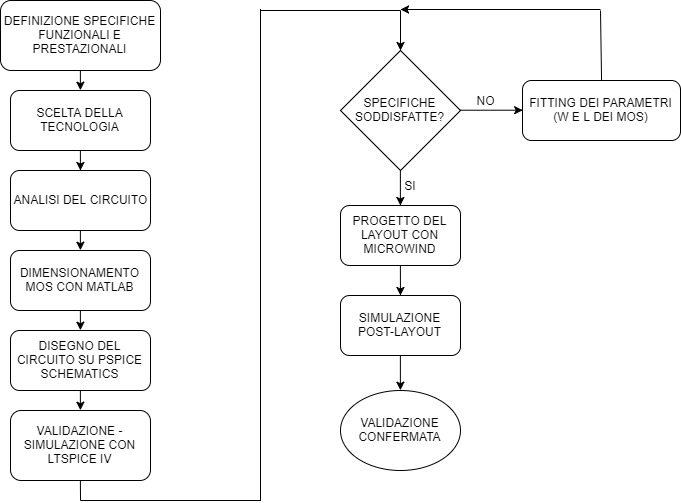
\includegraphics[width=0.7\textwidth]{figure/Workflow.jpg}
	\caption{Flusso di processo.}
	\label{fig:workflow}
\end{figure}









% Chapter 1

\chapter{Analisi} % Write in your own chapter title
\label{Chapter2}
\lhead{\emph{Analisi}}

\section{Il modello del MOS}
\label{sec:sec_mos}

Dato che il circuito trattato in questo progetto è basato su tecnologia CMOS è doveroso iniziare con l'analisi del \textit{mattoncino base} che lo compone, ossia il transistor di tipo MOSFET.

In Fig. \ref{fig:simboliMos} il simbolo per un NMOS.

\begin{figure}[hbt!]
	\centering
	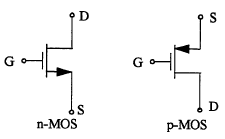
\includegraphics[width=0.5\textwidth]{figure/simboliMos.png}
	\caption{Simbolo NMOS (a sinistra) e PMOS (a destra)}
	\label{fig:simboliMos}
\end{figure}

L'eq. \ref{eq:eq_MOS_zonaSaturazione} descrive il comportamento di un MOS in zona di saturazione, impiegando un modello quadratico piuttosto semplificato:

\begin{equation}
	I_{D} = \frac{1}{2} \mu _{n} C^{'}_{ox} \frac{W}{L} (V_{GS}-V_{th})^2
	\label{eq:eq_MOS_zonaSaturazione}
\end{equation}

ed è valida quando $V_{DS} > V_{GS}-V_{th}$.

\section{La caratteristica reale del MOS}
\label{sec:sec_caratteristicaMOS}
Il modello del MOS mostrato nella sezione \ref{sec:sec_mos} è ben distante dalla realtà, perché si manifestano:
\begin{itemize}
	\item \textit{effetti di canale corto}, particolarmente visibili quando i transistor sono realizzati con la lunghezza minima disponibile per la tecnologia, come nel caso dei dispositivi digitali, in cui si vogliono minimizzare le dimensioni; ciò comporta la progressiva riduzione della velocità dei portatori di carica nel canale, diminuendo il fattore $\mu$ e quindi il guadagno;
	\item \textit{effetto body}, per il quale la $V_{th}$ diminuisce all'aumentare della tensione $V_{SB}$; nei dispositivi integrati spesso il source del MOS non è collegato al bulk (ovvero il substrato) e quindi $V_{SB} \neq 0 \Rightarrow \left | V_{th} \right | < \left | V_{th_0} \right | $ (con $V_{th_0}$ tensione di soglia per $V_{SB}=0$).
\end{itemize}

Utilizzando il software \textit{Microwind} e il simulatore \textit{LTspice} abbiamo ottenuto varie curve caratteristiche per confrontare il risultato più vicino alla realtà con quello aderente al modello teorico presentato in sezione \ref{sec:sec_mos}.

\section{Funzionamento dinamico dei circuiti CMOS}

Per valutare le prestazioni dinamiche della tecnologia CMOS, consideriamo come caso di studio un inverter con carico capacitivo ed effettuiamo un'analisi temporale fornendo in ingresso un'onda quadra.

\begin{figure}[hbt!]
	\centering
	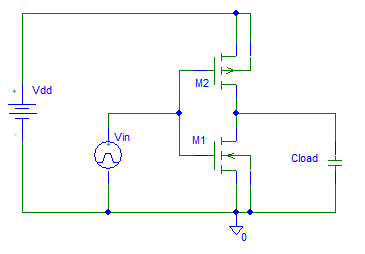
\includegraphics[width=0.5\textwidth]{figure/Sch_InverterCMOS.PNG}
	\caption{Inverter CMOS con capacità di carico.}
	\label{fig:fig_sch_inverterCMOS}
\end{figure}

\begin{figure}[hbt!]
	\centering
	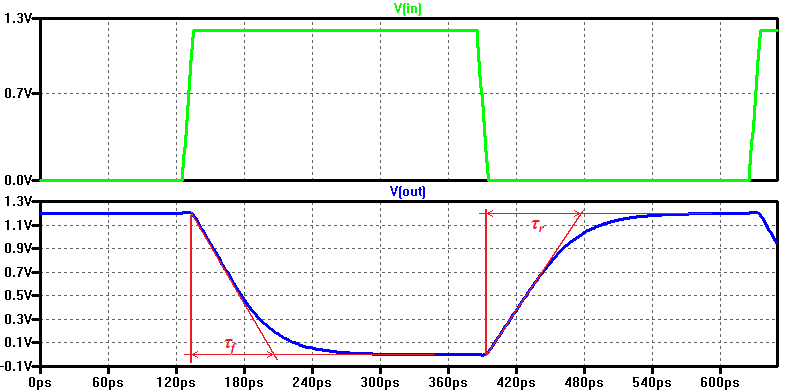
\includegraphics[width=1\textwidth]{figure/Sim_InverterCMOS(chiaro)WithNotes.png}
	\caption{Simulazione temporale di un inverter CMOS con capacità di carico.}
	\label{fig:fig_sim_inverterCMOS}
\end{figure}

Consideriamo un fronte di discesa della tensione d'uscita: in questo caso il condensatore, precedentemente caricato a $V_{DD}$ viene scaricato dal nMOS che funziona inizialmente in regime di saturazione ($V_{DS}>V_{GS}-V{th_n}$) per poi concludere la scarica in zona lineare. 

\begin{figure}[hbt!]
	\centering
	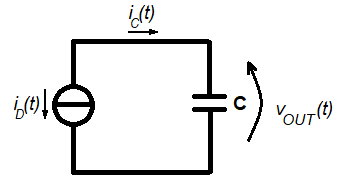
\includegraphics[width=0.4\textwidth]{figure/Sch_scaricaC.png}
	\caption{circuito equivalente per la scarica della capacità.}
	\label{fig:fig_sch_scaricaC}
\end{figure}

Questa situazione è schematizzata in figura \ref{fig:fig_sch_scaricaC}. La corrente $i_D(t) = - i_C(t)$ è quella che scorre nel canale del nMOS scaricando il condensatore. Si ha che:
\begin{equation}
i_C(t) = C \frac{d}{dt}v_{OUT}(t)
\label{eq:eq_condensatore}
\end{equation}
da cui, integrando tra $t_0$ e $t$, si ottiene l'evoluzione temporale di $v_{OUT}(t)$ a partire dalla condizione iniziale $v_{OUT}(t_0)$:
\begin{equation}
\int_{t_0}^{t} i_C(\xi)\, d\xi = C \int_{t_0}^{t} \frac{d}{d\xi}v_{OUT}(\xi)\, d\xi
\label{eq:eq_condensatoreIntegrata}
\end{equation}
ovvero, calcolando l'integrale a secondo membro e riordinando i termini:
\begin{equation}
v_{OUT}(t) - v_{OUT}(t_0) = \frac{1}{C}\int_{t_0}^{t} i_C(\xi)\, d\xi
\label{eq:eq_condensatoreSoluzione}
\end{equation}
Un'approssimazione valida per semplificare l'analisi si ottiene supponendo che il transistor operi solo in saturazione; esso si comporta quindi come un generatore di corrente costante e $i_C(t) = - i_D(t) = - I_D$; in tal caso l'integrale a secondo membro diventa una retta in $t$ e la scarica di $C$ ha un andamento lineare:

\begin{equation}
v_{OUT}(t) - v_{OUT}(t_0) \approx - \frac{1}{C}\int_{t_0}^{t} I_D \, d\xi = - \frac{I_D}{C}(t - t_0)
\label{eq:eq_condensatoreSoluzioneLineare}
\end{equation}

Questa formula, chiaramente, ha senso fisico finché $0 < V_{out}(t) < V_{DD}$, ovvero per i $t$ che soddisfano questo vincolo. Scegliendo un istante di tempo $t_1 > t_0$, si ha:
\begin{equation}
\Delta V = \left | v_{OUT}(t_1) - v_{OUT}(t_0) \right | \approx \frac{\left | I_D \right | }{C}(t_1 - t_0)
\label{eq:eq_condesatoreLineare}
\end{equation}

Nel caso del fronte di salita conduce il pMOS e si possono fare considerazioni analoghe; la \ref{eq:eq_condesatoreLineare} resta valida grazie agli operatori di valore assoluto.

Ai fini progettuali, in riferimento ai fronti di salita e discesa siamo interessati al tempo necessario per passare dal livello logico basso ($0V$) a quello alto  ($+V_{DD}$) e viceversa. Nel caso di fronte di discesa, iniziamo l'analisi con $C$ carico a $v_{OUT}(t_0) = V_{DD}$ e scegliamo $t_1 \ t.c. \ v_{OUT}(t_1) = 0$; facciamo il viceversa con il fronte di salita. Otteniamo così una comoda formula approssimata, valida in entrambi i casi:
\begin{equation}
\Delta V = \frac{\tau \left | I_D \right |}{C} \qquad \Leftrightarrow \qquad \left | I_D \right | = C \frac{\Delta V}{\tau}
\label{eq:eq_condensatoreLineareFinale}
\end{equation}
dove $\Delta V = V_{DD}$ è (in modulo) il "salto" di tensione da compiere e $\tau := t_1 - t_0$ è una stima del tempo di salita/discesa, ovvero il tempo di carica/scarica (lineare) della capacità $C = C_{load}$.

La validità di questa formula è discutibile: la stima del tempo di discesa è ottimistica ma è comunque utilizzabile come riferimento grossolano ai fini progettuali. Infatti, unendo questo risultato con l'equazione \ref{eq:eq_MOS_zonaSaturazione} (corrente di drain del MOS in saturazione) si ottiene una formula di progetto approssimata per determinare il rapporto d'aspetto necessario per avere i desiderati tempi di salita e discesa:

\begin{equation}
\frac{W}{L} =
\begin{dcases}
\frac{2 \ C_{load} \ V_{DD}}{\tau \mu _{n} C^{'}_{ox} (V_{DD}-V_{thn})^2} \quad nMOS\\
\frac{2\ C_{load} \ V_{DD}}{\tau \mu _{p} C^{'}_{ox} (V_{DD}-|V_{thp}|)^2} \quad pMOS
\end{dcases}
\label{eq:formulaRapportoAspetto}
\end{equation}

Una rappresentazione della carica/scarica lineare confrontata con l'andamento reale è visibile in figura \ref{fig:fig_sim_inverterCMOS}.

\section{Il Full Adder TSPC}
\label{sec:sec_fullAdder}








% Chapter 1

\chapter{Progettazione circuitale} % Write in your own chapter title
\label{Chapter3} 
\lhead{\emph{Progettazione circuitale}}

\section{Schema completo}
\begin{figure}[hbt!]
	\centering
	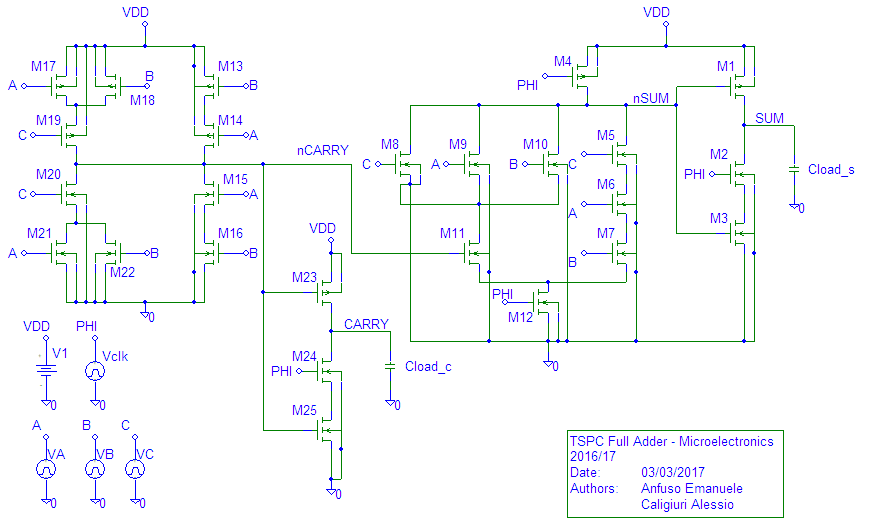
\includegraphics[width=1\textwidth]{figure/TSPC_FA_SchematicScreen.png}
	\caption{Schema completo del full-adder.}
	\label{fig:schemaCircuitale}
	\end{figure}
In fig. \ref{fig:schemaCircuitale} è mostrato lo schema completo del full-adder, così come simulato in \textit{SPICE}. Tutti i \textit{bulk} degli nMOS e dei pMOS sono stati collegati rispettivamente a massa e all'alimentazione positiva, in modo tale da assicurare la polarizzazione inversa delle giunzioni \textit{bulk - drain} e \textit{bulk - source} in ogni condizione operativa. Questa scelta è inoltre obbligata dalla realizzazione su silicio nella quale tutti i bulk degli nMOS (pMOS) corrispondono al medesimo substrato di tipo \textit{p} ("vasca" \textit{n-well}).

\section{Dimensionamento di massima}
\label{sec:sec_dimensionamentoMassima}
Il dimensionamento dei transistor prevede di iniziare dagli \textbf{stadi finali} \textit{2.2} e \textit{3} (in riferimento alla fig. \ref{fig:fig_schemaDaArticoloStadiCerchiati}), relativi rispettivamente ai MOS \textit{M1, M2, M3} e\textit{ M23, M24, M25} dello schema in fig. \ref{fig:schemaCircuitale}; entrambi hanno una capacità di carico $C_{load} = 100fF$, fornita dalle specifiche indicate in sezione \ref{sec:sec_fasiLavoro}.

Le capacità di gate di \textit{M1} e \textit{M3} costituiranno il carico dello stadio \textit{2.1} precedente; dipendendo queste dalle dimensioni dei MOS, si giustifica la necessità di iniziare dai finali e tornare indietro.
Si osservi che analogamente il carico dello stadio \textit{1} è dato dal parallelo delle capacità di gate di \textit{M23}, \textit{M25} (stadio \textit{2.2}) e \textit{M11} (stadio \textit{2.1}).

\subsection{Vincoli temporali e \textit{inverter equivalente}}
\label{subsec:specifiche}
Dalla frequenza operativa richiesta di $f_{clock} = 2GHz$ (ovvero periodo $T_{clock} = 500ps$) derivano vincoli temporali sulle fasi di valutazione e precarica, che devono andare a regime entro $T_{clock}/2 = 250ps$. Rispetto al formalismo usato in sezione \ref{sec:funzionamentoDinamicoCMOS}, questo vuol dire che i tempi di salita e di discesa dei singoli stadi devono restare entro tale limite: 
\begin{equation}
	\tau = \tau_{r} = \tau_{f} < T_{clock}/2 = 250ps
\end{equation}

A titolo precauzionale si fissa $\tau = 200ps$, tenendo conto anche dei $25ps$ dati come tempi di salita/discesa delle tensioni \textit{A, B, C, clock} in ingresso.

A questo punto si può applicare la formula \ref{eq:formulaRapportoAspetto}, impiegando i valori di $\mu _n$, $\mu _p$ e $C'_{ox}$ trovati in sezione \ref{sec:sec_mos}, ottenendo così i \textbf{rapporti d'aspetto dei MOS di un \textit{inverter equivalente}} che deve pilotare la data capacità di carico completando la carica entro il tempo definito. Si ricorda nuovamente che il risultato fornito da questa formula è decisamente più piccolo del necessario, a causa di approssimazioni ottimistiche sia sul tempo di carica/scarica (assunta lineare per facilità) sia sulla caratteristica del MOS, come già discusso.

\subsection{Dall'\textit{inverter equivalente} alle dimensioni dei MOS}
\label{subsec:daInverterAMOS}
Ai fini progettuali, ogni stadio del full-adder è assimilabile ad un \textit{inverter equivalente} dal momento che il segnale in uscita è \textit{alzato} a $V_{DD}$ da una serie/parallelo di pMOS ed \textit{abbassato} a massa da una serie/parallelo di nMOS; per ragioni geometriche entrambe queste combinazioni di transistor possono essere ricondotte ad un singolo componente di dimensioni opportune, considerando il caso peggiore.

Consideriamo per esempio la parte superiore dello stadio \textit{1}. Il percorso di corrente più sfavorevole si ha quando conducono solo \textit{M13} e \textit{M14} (o, analogamente, solo \textit{M17} e \textit{M19}). Due \textbf{MOS di uguale larghezza in serie} si possono valutare come un unico MOS con \textbf{rapporto d'aspetto equivalente} ridotto, come mostra la figura seguente.

\begin{figure}[hbt!]
	\centering
	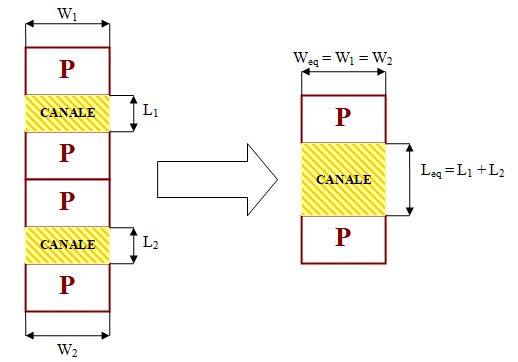
\includegraphics{figure/PMOS_series.png}
	\caption{Considerazioni geometriche sulle dimensioni di due pMOS in serie.}
	\label{fig:PMOS_series}
\end{figure}

Quando entrambi i transistor sono in conduzione, la corrente di drain percorre due canali, per una lunghezza totale $L_{eq} = L_1 + L_2$ e una larghezza costante $W_{eq} = W_1 = W_2 = W$. Se i due MOS hanno anche lunghezza di canale uguale ($L=L_1 = L_2$), il rapporto d'aspetto risulta dimezzato; infatti:
\begin{equation}
	\left ( \frac{W}{L} \right ) _{eq} = \frac{W}{L_1 + L_2} = \frac{W}{2 \cdot L} =  \frac{\left ( \frac{W}{L} \right ) _{1}}{2} = \frac{\left ( \frac{W}{L} \right ) _{2}}{2} 
\end{equation}
Questo vale sia per dispositivi a canale \textit{n} che a canale \textit{p}.
In generale, si può affermare che, con un numero $n \in  \mathbb{N}$ di MOS tutti uguali in serie, il rapporto d'aspetto del transistor equivalente è:
\begin{equation}
\left ( \frac{W}{L} \right ) _{eq} = \frac{\left ( \frac{W}{L} \right )}{n} 
\end{equation}
Una considerazione duale si può fare considerando il parallelo di MOS uguali, nel qual caso il rapporto d'aspetto del singolo è moltiplicato per il numero di dispositivi. Tuttavia questa considerazione non è d'interesse nella circostanza considerata, in quanto il caso peggiore in un parallelo si ha sempre quando conduce un solo MOS alla volta.

Per brevità non si riportano i conti sui singoli stadi, rimandando l'analisi degli stessi ai relativi script \textit{MATLAB}.

\subsection{Dimensioni geometriche dei MOS: risultati di \textit{MATLAB}}

Di seguito si riportano le dimensioni di massima dei MOS ottenute applicando le considerazioni precedenti; tali risultati sono stati calcolati con alcuni script \textit{MATLAB}.

\begin{table}[htb]
	\centering
	\begin{tabular}{c*{5}{c}}
		\toprule
		MOS & Canale & $W/L$ & W($\mu$m) & L($\mu$m) & Stadio\\
		\midrule
		M1 & p & 10 & 1.20 & 0.12 & Finale \textit{SUM} \\
		M2, M3 & n & 6 & 0.72 & 0.12 & " \\
		M4 & p & 2 & 0.24 & 0.12 & Generazione \textit{!SUM} \\
		M5, M6, M7 & n & 2 & 0.24 & 0.12 & " \\
		M8, M9, M10 & n & 2 & 0.24 & 0.12 & " \\
		M11 & n & 2 & 0.24 & 0.12 & " \\
		M12 & n & 2 & 0.24 & 0.12 & " \\
		M13, M14 & p & 6 & 0.72 & 0.12 & Generazione \textit{!CARRY} \\
		M15, M16 & n & 2 & 0.24 & 0.12 & " \\
		M17, M18, M19 & p & 6 & 0.72 & 0.12 & " \\
		M20, M21, M22 & n & 2 & 0.24 & 0.12 & " \\
		M23 & p & 8 & 0.96 & 0.12 & Finale \textit{CARRY} \\
		M24, M25 & n & 5 & 0.60 & 0.12 & " \\
		\bottomrule
	\end{tabular}
	\caption{Tabella delle dimensioni calcolate dei MOS, non valide.}
	\label{tab:dimensioniMosTeoriche}
\end{table}

\subsection{Prima simulazione \textit{pre-layout}}
La prima simulazione \textit{SPICE} (fig. \ref{fig:primaSimulazionePreLayout}) del circuito dimensionato come da tabella \ref{tab:dimensioniMosTeoriche} ha restituito dei risultati imbarazzanti: i segnali in uscita \textit{SUM} (in blu) e \textit{CARRY} (in verde) spesso non riescono a raggiungere le tensioni di alimentazione, perché le commutazioni sono troppo lente.

\begin{figure}[hbt!]
	\centering
	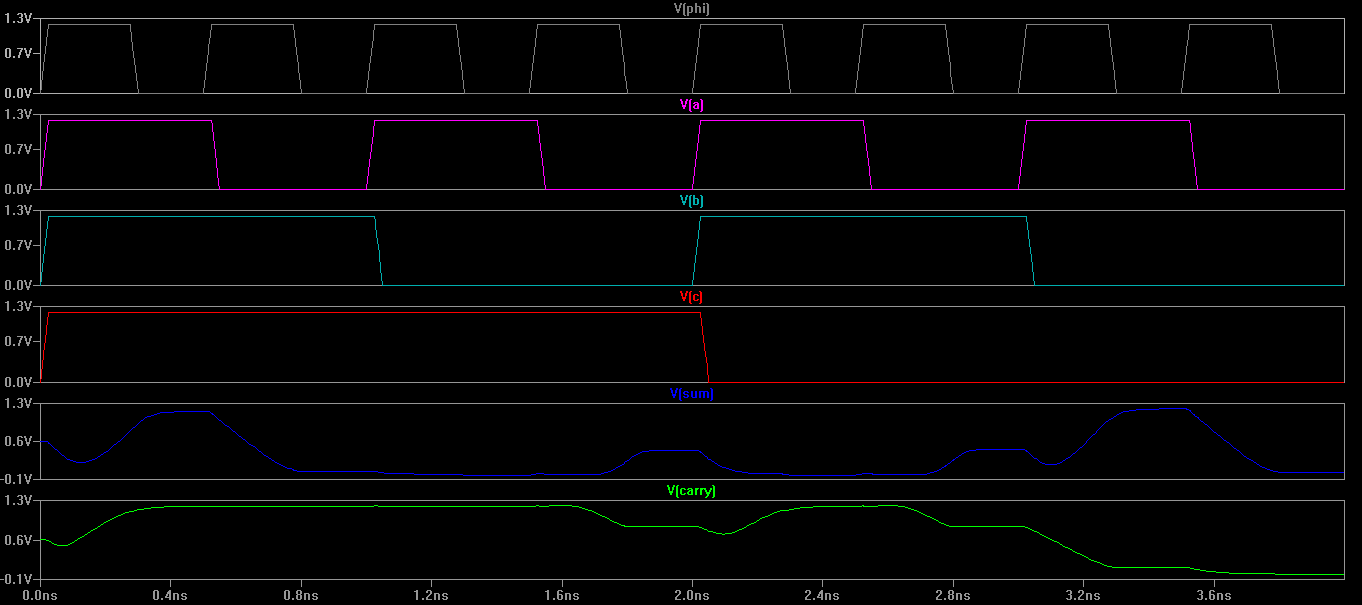
\includegraphics[width=1.3\textwidth, angle=90]{figure/sim_FA_Bad.png}
	\caption{Prima simulazione \textit{pre-layout} con dimensioni calcolate dei MOS.}
	\label{fig:primaSimulazionePreLayout}
\end{figure}

Per comprendere le cause di questo fallimento, abbiamo provato ad ingannare il simulatore semplificando il modello del MOS, esattamente come in sezione \ref{sec:ilModelloDiMicrowind}. Ne è risultata una simulazione, qui omessa, decisamente più aderente ai risultati attesi che ha testimoniato la bontà del dimensionamento effettuato ma chiaramente non attendibile dal momento che non ricalca il reale funzionamento dei MOS. Ad esempio, a causa del forte campo elettrico nella zona di canale dovuto alle ridotte dimensioni dei MOS (tutti a lunghezza minima), $\mu_n$ e $\mu_p$ non sono più costanti e diminuiscono rispetto ai valori calcolati, come già discusso in sezione \ref{sec:sec_caratteristicaMOS}.



\section{Fitting dei parametri: dimensioni definitive}
\label{sec:sec_fittingParametri}
Al fine di ottenere delle formule di progetto adeguate, sarebbe alquanto arduo utilizzare per i MOS il modello matematico \textit{SPICE level 3}. Abbiamo inizialmente provato a ricavare $\mu \cdot C'_{ox}$ e $V_{th}$ dalle curve caratteristiche \textit{level 3} di fig. \ref{fig:curveCaratteristicheReali} per utilizzare questi valori nella formula \ref{eq:formulaRapportoAspetto}, ottenendo dei transistor di larghezza assai elevata vista l'applicazione in questione.
Pertanto abbiamo scelto di cambiare approccio e operare in modo empirico: dopo un'attenta analisi dei segnali intermedi ottenuti mediante simulazioni, abbiamo agito sulle singole dimensioni dei transistor critici e, per approssimazioni successive, ci siamo avvicinati ad una soluzione soddisfacente sia dal punto di vista temporale che geometrico.

\MakeUppercase{è} stato necessario aumentare le dimensioni dei singoli transistor, in particolare di quelli finali che pilotano le uscite \textit{SUM} e \textit{CARRY} (stadi \textit{3} e \textit{2.2}). La tabella seguente riporta le nuove dimensioni.

\begin{table}[htb]
	\centering
	\begin{tabular}{c*{5}{c}}
		\toprule
		MOS & Canale & $W/L$ & W($\mu$m) & L($\mu$m) & Stadio\\
		\midrule
		M1 & p & 30 & 3.60 & 0.12 & Finale \textit{SUM} \\
		M2, M3 & n & 16 & 1.92 & 0.12 & " \\
		M4 & p & 10 & 1.20 & 0.12 & Generazione \textit{!SUM} \\
		M5, M6, M7 & n & 16 & 1.92 & 0.12 & " \\
		M8, M9, M10 & n & 10 & 1.20 & 0.12 & " \\
		M11 & n & 10 & 1.20 & 0.12 & " \\
		M12 & n & 16 & 1.92 & 0.12 & " \\
		M13, M14 & p & 24 & 2.88 & 0.12 & Generazione \textit{!CARRY} \\
		M15, M16 & n & 8 & 0.96 & 0.12 & " \\
		M17, M18, M19 & p & 24 & 2.88 & 0.12 & " \\
		M20, M21, M22 & n & 8 & 0.96 & 0.12 & " \\
		M23 & p & 30 & 3.60 & 0.12 & Finale \textit{CARRY} \\
		M24, M25 & n & 20 & 2.40 & 0.12 & " \\
		\bottomrule
	\end{tabular}
	\caption{Tabella delle dimensioni dei MOS dopo il \textit{fitting}.}
	\label{tab:dimensioniMosDefinitive}
\end{table}

\subsection{Simulazione \textit{pre-layout} soddisfacente}
La simulazione \textit{SPICE} \textit{pre-layout} finale mostra un corretto funzionamento del circuito. \MakeUppercase{è} agevole verificare che a fronte degli ingressi \textit{A}, \textit{B}, \textit{C}, le uscite \textit{SUM} e \textit{CARRY} forniscono i corretti valori logici e tensioni accettabili.

\begin{figure}[hbt!]
	\centering
	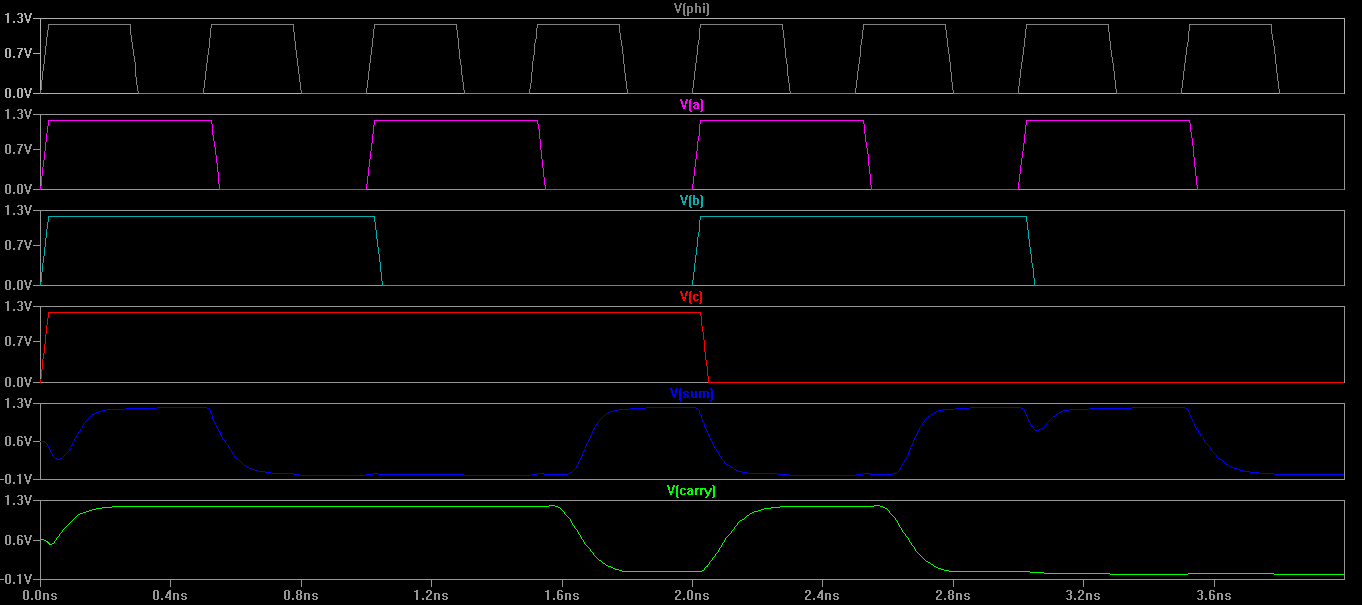
\includegraphics[width=1.5\textwidth, angle=90]{figure/sim_FA_Good.png}
	\caption{Simulazione \textit{pre-layout} soddisfacente.}
	\label{fig:simulazionePreLayoutSoddisfacente}
\end{figure}

Sarà necessario eseguire un'analoga simulazione \textit{post-layout}, ovvero dopo il disegno su silicio del circuito.
% Chapter 4

\chapter{Layout} % Write in your own chapter title
\label{Chapter4} 
\lhead{\emph{Layout}}

In Fig. \ref{fig:layout} si può ammirare il layout finale del Full Adder TSPC.

\begin{figure}[hbt!]
	\centering
	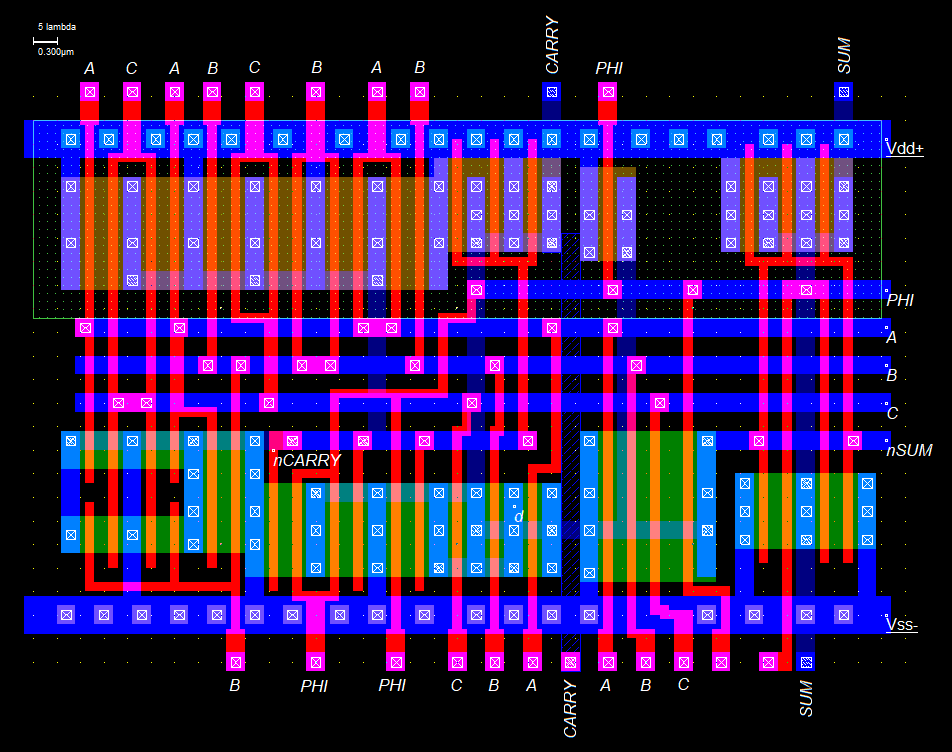
\includegraphics[width=1\textwidth]{figure/Msk_FullDesign.png}
	\caption{Layout finale.}
	\label{fig:layout}
\end{figure}

Vediamo quali sono stati i passi che hanno portato alla sua realizzazione.

\section{Disegno dei singoli stadi}
\label{sec:sec_disegnoStadi}

Un possibile metodo di lavoro prevede di ottenere il circuito finale in maniera progressiva, realizzando e validando un singolo stadio alla volta, mediante simulazioni \textit{post-layout}. Il circuito finale è ottenuto dall'unione dei vari pezzi ed è a sua volta validato da una simulazione dello stesso tipo che, se soddisfacente, sancisce il raggiungimento degli obiettivi prefissati. 

Analizziamo quindi i disegni delle singole parti di circuito riportando alcuni screen tratti da \textit{Microwind} e i cui colori hanno i seguenti significati:

\begin{itemize}
	\item lo sfondo nero rappresenta il substrato di tipo \textit{p};
	\item le aree verdi sono diffusioni di tipo \textit{n};
	\item le aree verdi a puntini sono diffusioni di tipo \textit{n-well};
	\item le aree rosse costituiscono piste di polisilicio;
	\item le aree blu sono metalizzazioni di tipo \textit{metal 1}; 
	\item i quadrati con la croce all'interno indicano la presenza di un contatto tra livelli differenti.
\end{itemize}

\subsection{Stadio \textit{1} - Generazione di !CARRY}

In fig. \ref{fig:NMOSePMOSnotCarry} si può osservare la realizzazione della parte \textit{n} (a sinistra) e della parte \textit{p} (a destra) dello stadio \textit{1} dedicato alla generazione del segnale \textit{!CARRY}, indicato nel layout con la label \textit{notCarry}. I MOS più larghi sono disegnati "ripiegati" su se stessi in modo da mantenere le dimensioni di canale desiderate pur potendo riorganizzare la disposizione delle diffusioni per meglio adattarsi alla forma generale che si vuole far assumere al circuito. 

Per ciascuno dei due circuiti viene estratta la netlist che, tramite \textit{LTspice}, permette di validare il disegno tenendo conto di tutti i parametri presenti nel modello della tecnologia utilizzata, incluse le capacità parassite.

\begin{figure}[hbt!]
	\centering
	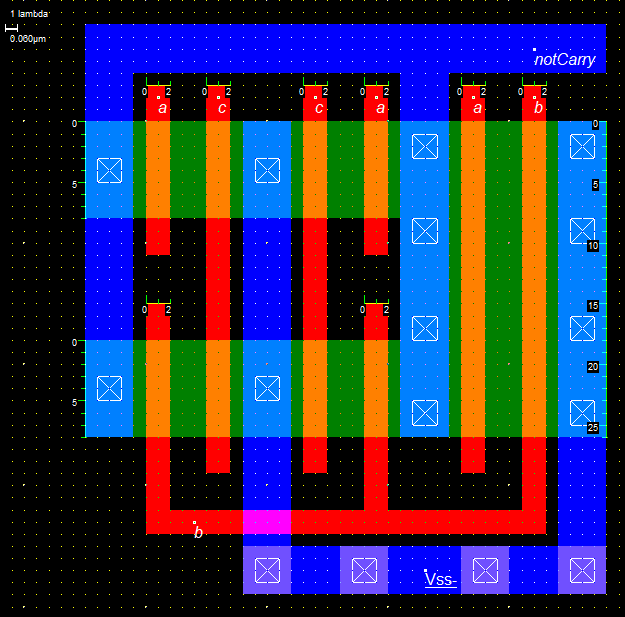
\includegraphics[width=0.4\textwidth]{figure/Msk_NMOS_notCarry_V2.png}\hfil
	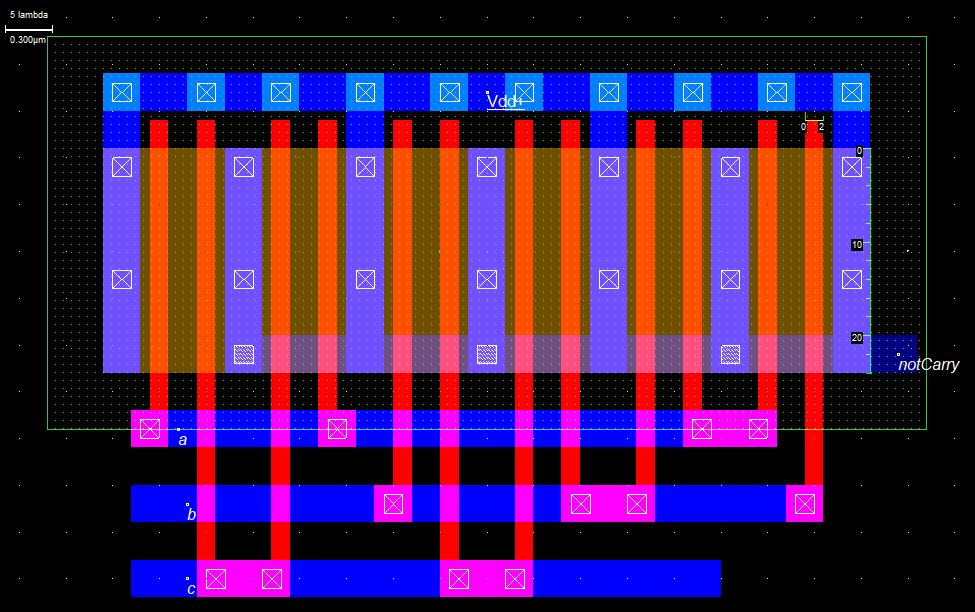
\includegraphics[width=0.4\textwidth]{figure/Msk_PMOS_notCarry_V2.png}
	\caption{Parte \textit{n} (a sinistra) e parte \textit{p} (a destra) dello stadio 1.}
	\label{fig:NMOSePMOSnotCarry}
\end{figure} 

Le due parti collegate costituiscono il disegno complessivo dello stadio \textit{1}, riportato in fig. \ref{fig:notCarry}. Da tale figura si può notare la scelta di adottare un approccio \textit{standard cell} per la disposizione delle piste di alimentazione e di segnale, come d'altronde viene suggerito nelle specifiche di progetto. In alto e in basso sono quindi presenti due piste orizzontali di \textit{Metal 1} collegate rispettivamente all'alimentazione positiva e negativa. I segnali \textit{A}, \textit{B}, \textit{C} e \textit{notCarry} sono forniti e prelevati in verticale, tramite piste di polisilicio per i primi tre e una pista di \textit{Metal 2} per l'ultimo. Tutti e quattro, assieme a \textit{phi}, sono poi trasportati nel resto del circuito da alcune piste di \textit{Metal 1}, orizzontali, poste tra le parti \textit{n} e le parti \textit{p} di ogni stadio.

\begin{figure}[hbt!]
	\centering
	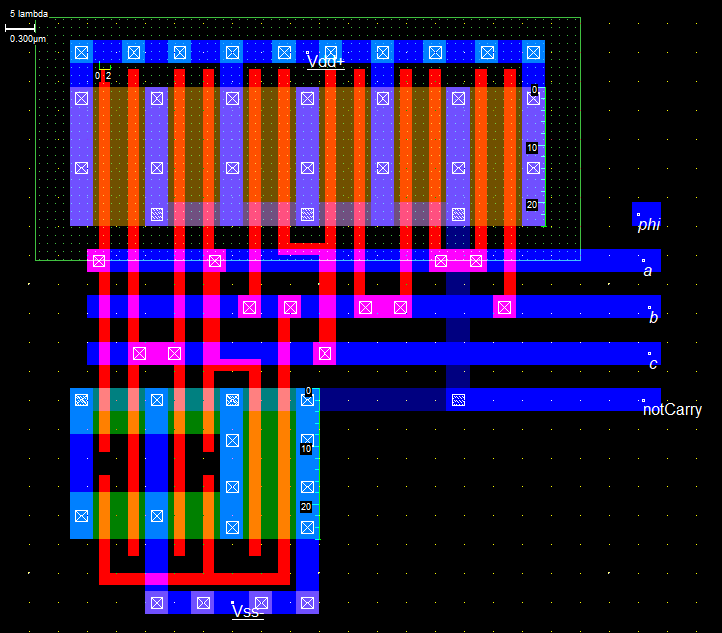
\includegraphics[width=0.5\textwidth]{figure/Msk_NotCarry_V2.png}
	\caption{Disegno dello stadio \textit{1} dedicato alla generazione di \textit{notCarry}.}
	\label{fig:notCarry}
\end{figure} 

Anche di questo circuito si effettua una simulazione \textit{post-layout} prima di procedere allo stadio successivo.

\subsection{Stadio \textit{2.1} - Generazione di !SUM}

In figura \ref{fig:NMOSnotSum} è riportato il disegno della parte \textit{n} dello stadio \textit{2.1} dedicato alla generazione del segnale \textit{!SUM}, etichettato come \textit{notSum}. Una particolarità di questa parte riguarda la realizzazione dei MOS in serie, ottenuta tramite l'affiancamento di diverse piste di polisilicio pilotate dai segnali d'ingresso; questa tecnica permette di risparmiare spazio evitando di inserire metalizzazioni per i gate dei MOS intermedi tra il nodo di uscita \textit{notSum} e il nodo comune ai due rami che compongono questa parte di circuito: non è infatti necessario prelevare tali segnali.

\begin{figure}[hbt!]
	\centering
	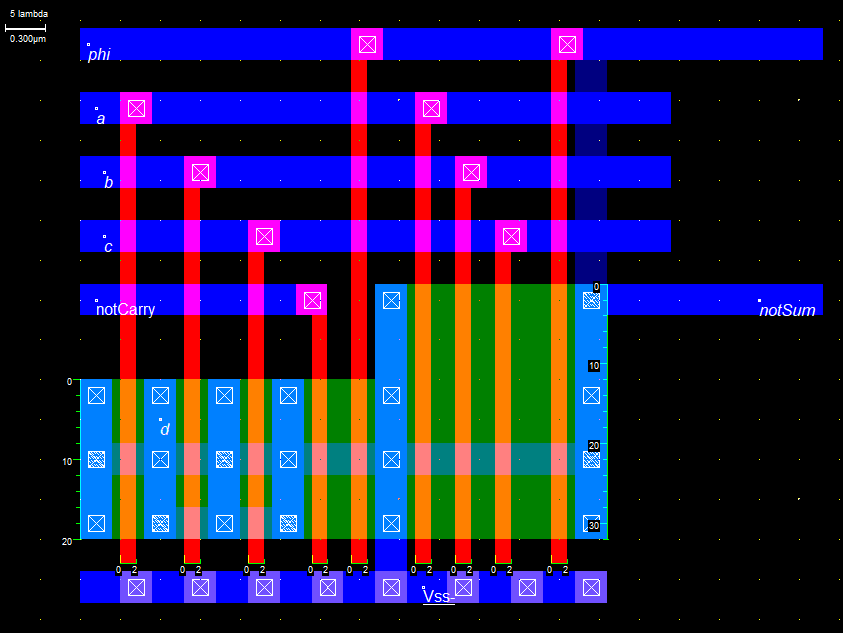
\includegraphics[width=0.5\textwidth]{figure/Msk_NMOS_NotSum.png}
	\caption{Parte \textit{n} dello stadio \textit{2.1} dedicato alla generazione di \textit{notSum}.}
	\label{fig:NMOSnotSum}
\end{figure} 

La parte \textit{p} di questo stadio è costituita da un semplice pMOS per cui se ne omette la rappresentazione completa. Considerazioni circa la tipologia di progetto \textit{standard cell} e la procedura di validazione sono analoghe a quelle esposte per lo stadio \textit{1}.

\subsection{Stadi finali \textit{2.2} e \textit{3} - Generazione di CARRY e SUM}

Gli stadi finali \textit{2.2} e \textit{3} hanno la stessa identica struttura, per cui per brevità si riporta in fig. \ref{fig:sum} il disegno del solo stadio \textit{3}, dedicato alla generazione del segnale d'uscita \textit{SUM}.

\begin{figure}[hbt!]
	\centering
	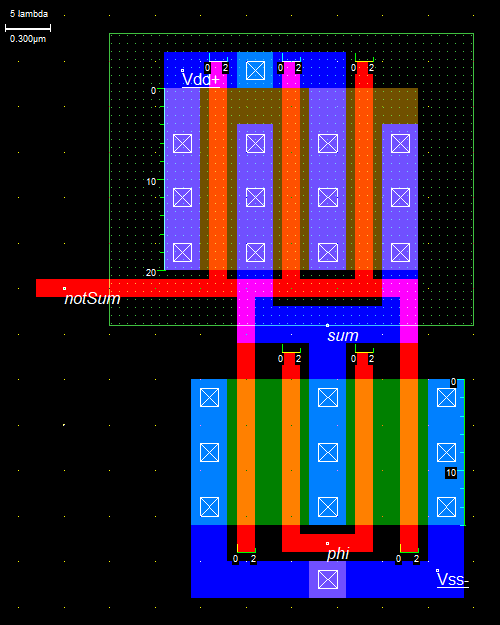
\includegraphics[width=0.5\textwidth]{figure/Msk_SumInveter.png}
	\caption{Disegno dello stadio \textit{3} dedicato alla generazione di \textit{SUM}.}
	\label{fig:sum}
\end{figure} 

Le tecniche utilizzate per il layout di questi stadi sono le stesse già presentate nei paragrafi precedenti. Terminata la sua validazione, si può procedere a comporre il circuito finale.

\section{Full design}
\label{sec:sec_fullDesign}

Il circuito finale, rappresentato in fig. \ref{fig:layout}, è il risultato della composizione dei singoli stadi presentati finora. Essi sono affiancati in modo da ottenere una struttura tanto più compatta possibile pur mantenendo la topologia delle varie parti. Ciò significa avvicinare le varie piste e/o diffusioni in modo da minimizzare gli spazi vuoti pur rispettando le regole di progettazione ovvero le distanze minime necessarie. 

Il risultato è un circuito molto ordinato e di dimensioni $11.04 \mu m \times 6.54 \mu m$ (ovvero, in \textit{lambda}, 184 x 109), con i segnali di ingresso/uscita prelevati e forniti in verticale e quelli di alimentazione applicati in orizzontale.

L'ultimo passo consiste nel compiere un'ultima validazione del circuito finale. Se ne esporta quindi la netlist che viene simulata tramite \textit{LTspice}. Il risultato della simulazione si osserva in fig. \ref{fig:simulazioneFinale}. Come si può notare a fronte di ogni combinazione degli ingressi \textit{A}, \textit{B}, \textit{C}, i segnali \textit{SUM} e \textit{CARRY} assumono il livello di tensione corretto entro le tempistiche richieste.  

\begin{figure}[hbt!]
	\centering
	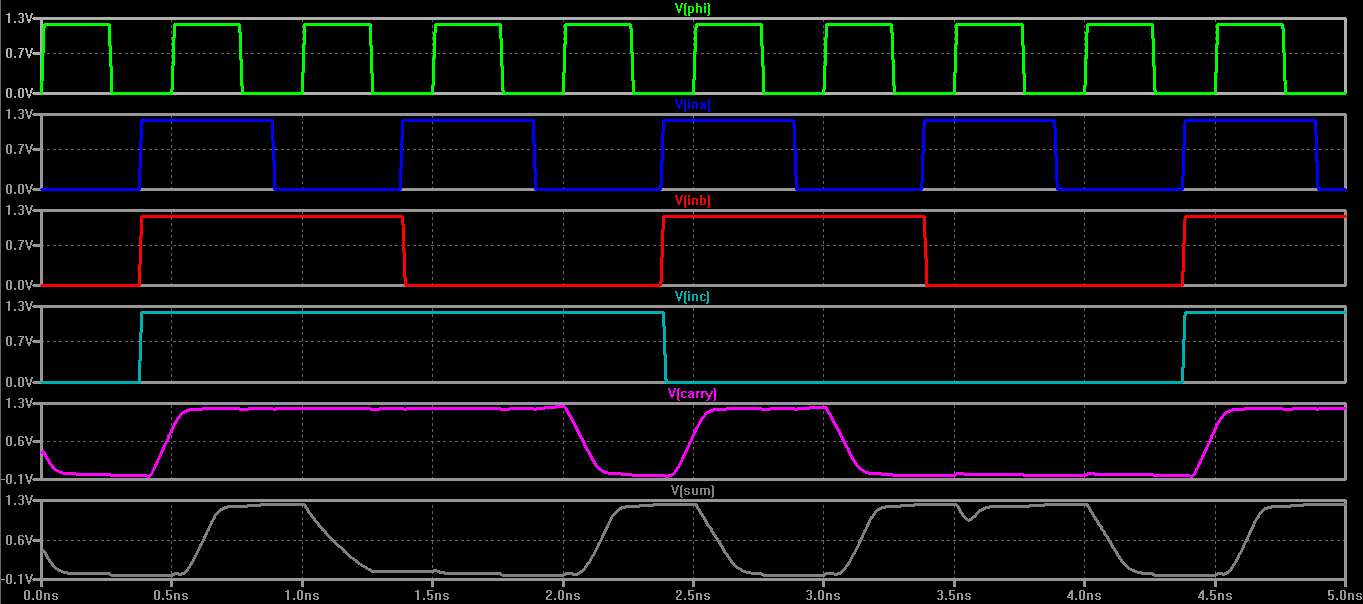
\includegraphics[width=1.5\textwidth, angle=90]{figure/Sim_FullDesign_PostLayout.PNG}
	\caption{Simulazione post-layout dello stadio finale.}
	\label{fig:simulazioneFinale}
\end{figure}

Da questa simulazione è anche possibile calcolare la potenza dissipata dal circuito in esame, che risulta pari a $315\mu W$.







% Chapter 5

\chapter{Conclusioni finali} % Write in your own chapter title
\label{Chapter5} 
\lhead{\emph{Conclusioni finali}}

In questo progetto abbiamo dunque realizzato un circuito Full Adder TSPC partendo dallo schema circuitale per ottenere come risultato finale il disegno delle maschere necessarie alla sua produzione.

La simulazione finale post-layout ha confermato che le specifiche richieste sono state soddisfatte. Inoltre la cura e l'attenzione riposte nella fase di stesura del layout hanno permesso di ottimizzare l'area finale e dunque la potenza dissipata.

Da un punto di vista formativo questo lavoro ci ha dato l'opportunità di imparare e adottare una metodologia di progetto chiara e completa. Abbiamo inoltre preso dimestichezza con alcuni software tipici della progettazione elettronica e ci siamo scontrati con alcune problematiche tipiche quando si parla della modellizzazione componenti fisici.









%% ----------------------------------------------------------------
% Now begin the Appendices, including them as separate files

%\addtocontents{toc}{\vspace{2em}} % Add a gap in the Contents, for aesthetics

%\appendix % Cue to tell LaTeX that the following 'chapters' are Appendices


%\addtocontents{toc}{\vspace{2em}}  % Add a gap in the Contents, for aesthetics
%\backmatter

%%%%%%%%%%%%%%%%%%%%%%%%%%%%%%%%%%%%%%%%%%%%%%%%%%%%%%%%%%%%%%%%%%
%
% BIBLIOGRAPHY
%
%%%%%%%%%%%%%%%%%%%%%%%%%%%%%%%%%%%%%%%%%%%%%%%%%%%%%%%%%%%%%%%%%%

%% ----------------------------------------------------------------
\label{Bibliography}
\lhead{\emph{Bibliography}}  % Change the left side page header to "Bibliography"
\bibliographystyle{unsrtnat}  % Use the "unsrtnat" BibTeX style for formatting the Bibliography
\bibliography{Bibliography}  % The references (bibliography) information are stored in the file named "Bibliography.bib"

\clearpage

%% ----------------------------------------------------------------
\setstretch{1.2}  % Reset the line-spacing to 1.3 for body text (if it has changed)


\end{document}  % The End